%!TEX root = ../report.tex

\chapter{Solution}


During this research and development project, a system was implemented which is able to record human demonstrations in terms of kinematic trajectory, learn the motion in terms of dynamic motion primitive, reproduce the motion using dynamic motion primitive and execute this motion on manipulator.     

\begin{figure}[H]
	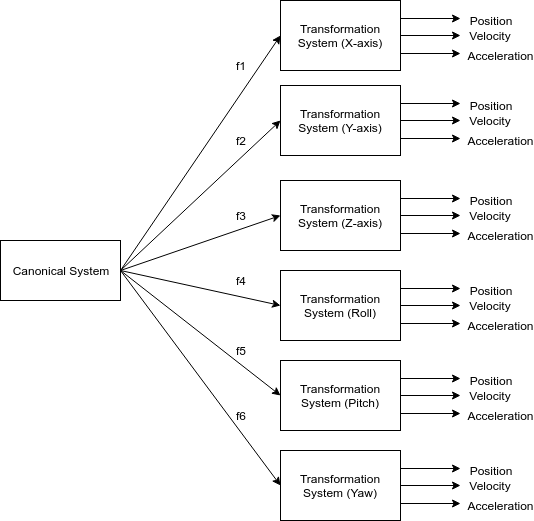
\includegraphics[width=\textwidth]{images/DMP_6DOF.png}
	\caption{6D DMP framework used during experimentation}
	\label{fig:DMP_6DOF}
\end{figure}


\section{Proposed algorithm}

\newpage
\begin{figure}[H]
	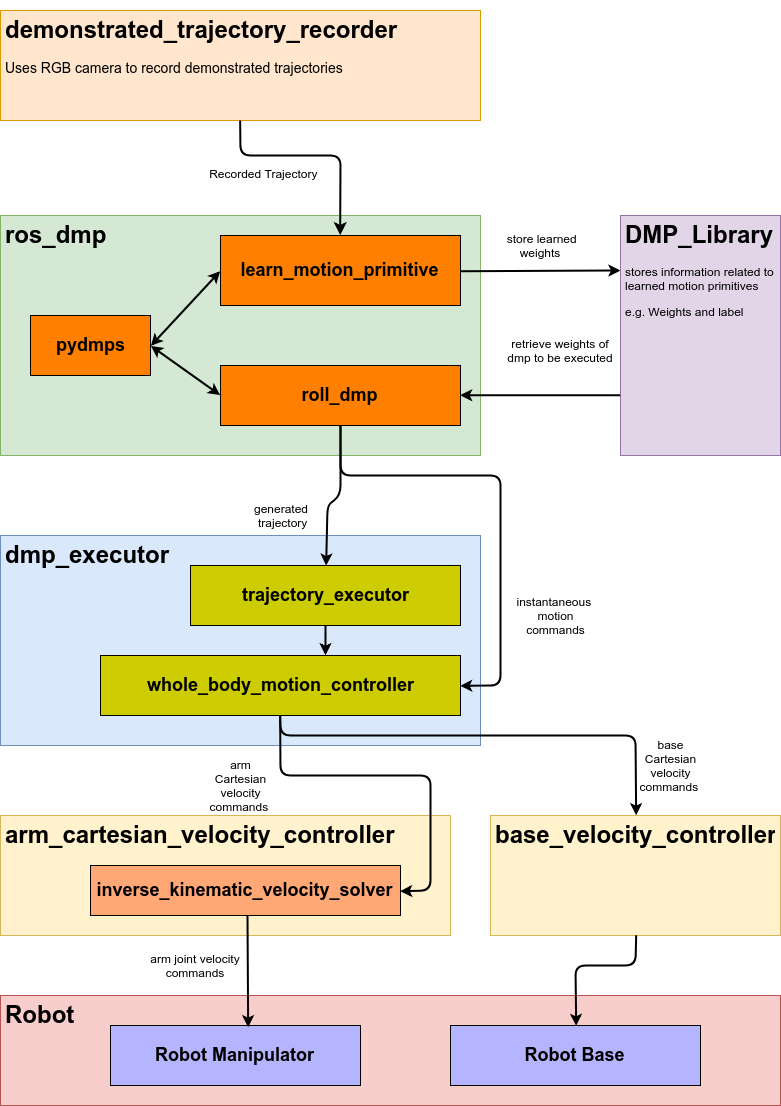
\includegraphics[width=\textwidth]{images/framework.png}
	\caption{Dynamic Movement Primitive framework}
	\label{fig:framework}
\end{figure}

\subsection{Whole Body Motion Control}

For the mobile manipulators like KUKA YouBot and Toyota HSR, it is always desirable to have a whole body control functionality i.e. executing motion using mobile base as well as manipulator in order to achieve a objective (e.g. attaining a particular end effector pose in global reference frame or executing a trajectory represented in global reference frame). Commonly used sampling based algorithms can be used to achieve this goal by providing model of environment as well as robot. Dynamic programming based approaches and optimization based motion planning can also solve the problem of whole body motion control, but they heavily suffer from the increased dimensionality of the problem. Prominent drawbacks of such methods are described below. 

While conducting the initial experiments on DMP framework with KUKA YouBot, we came across the serious problem of limited manipulation functionality of 5 degrees of freedom manipulator. Numerous trajectories demonstrated were not executable by manipulator alone. This triggered the idea of incorporating base movement to execute the manipulator motion. 


  

\section{Implementation details}

In order to use dynamic motion primitives in robotics, one has to demonstrate the motion to robot, learn the control policy using DMPs, reproduce the motion policy or trajectory and then execute the motion with robot. In this research and development project, motion trajectory is demonstrated using visual demonstrations with the help of arUco marker board. Since the trajectory is learned and reproduced in task space, it is mapped to joint space using kinematic solver and then executed on the robot. Above figure shows the architecture of the software implementation. Necessary components for above mentioned steps are as follows, 

\subsection{Demonstrated Trajectory Recorder}
Various methods for demonstrating trajectories are practiced by researchers mainly :
\begin{itemize} 
	
	\item Teleoperation : A demonstration technique in which the teacher operates the robot learner platform and the robot’s sensors record the execution. 	\cite{argall2009survey}	
	
	\item Shadowing : A demonstration technique in which the robot learner records the execution using its own sensors while attempting to match or mimic the teacher motion as the teacher executes the task.
	
	\item Sensors on teacher : An imitation technique in which sensors located on the executing body are used to record the teacher execution.
	
	\item External observation : An imitation technique in which sensors external to the executing body are used to record the execution.
	
\end{itemize}

In this project, \textit{external observation} method was used to demonstrate trajectories. Teacher demonstrated trajectories by moving arUco marker board on desired path. A computer vision system ensured the recording of poses of arUco marker board in robot \textit{base\_link} frame, at constant rate. 

\begin{figure}[H]
	\centering
	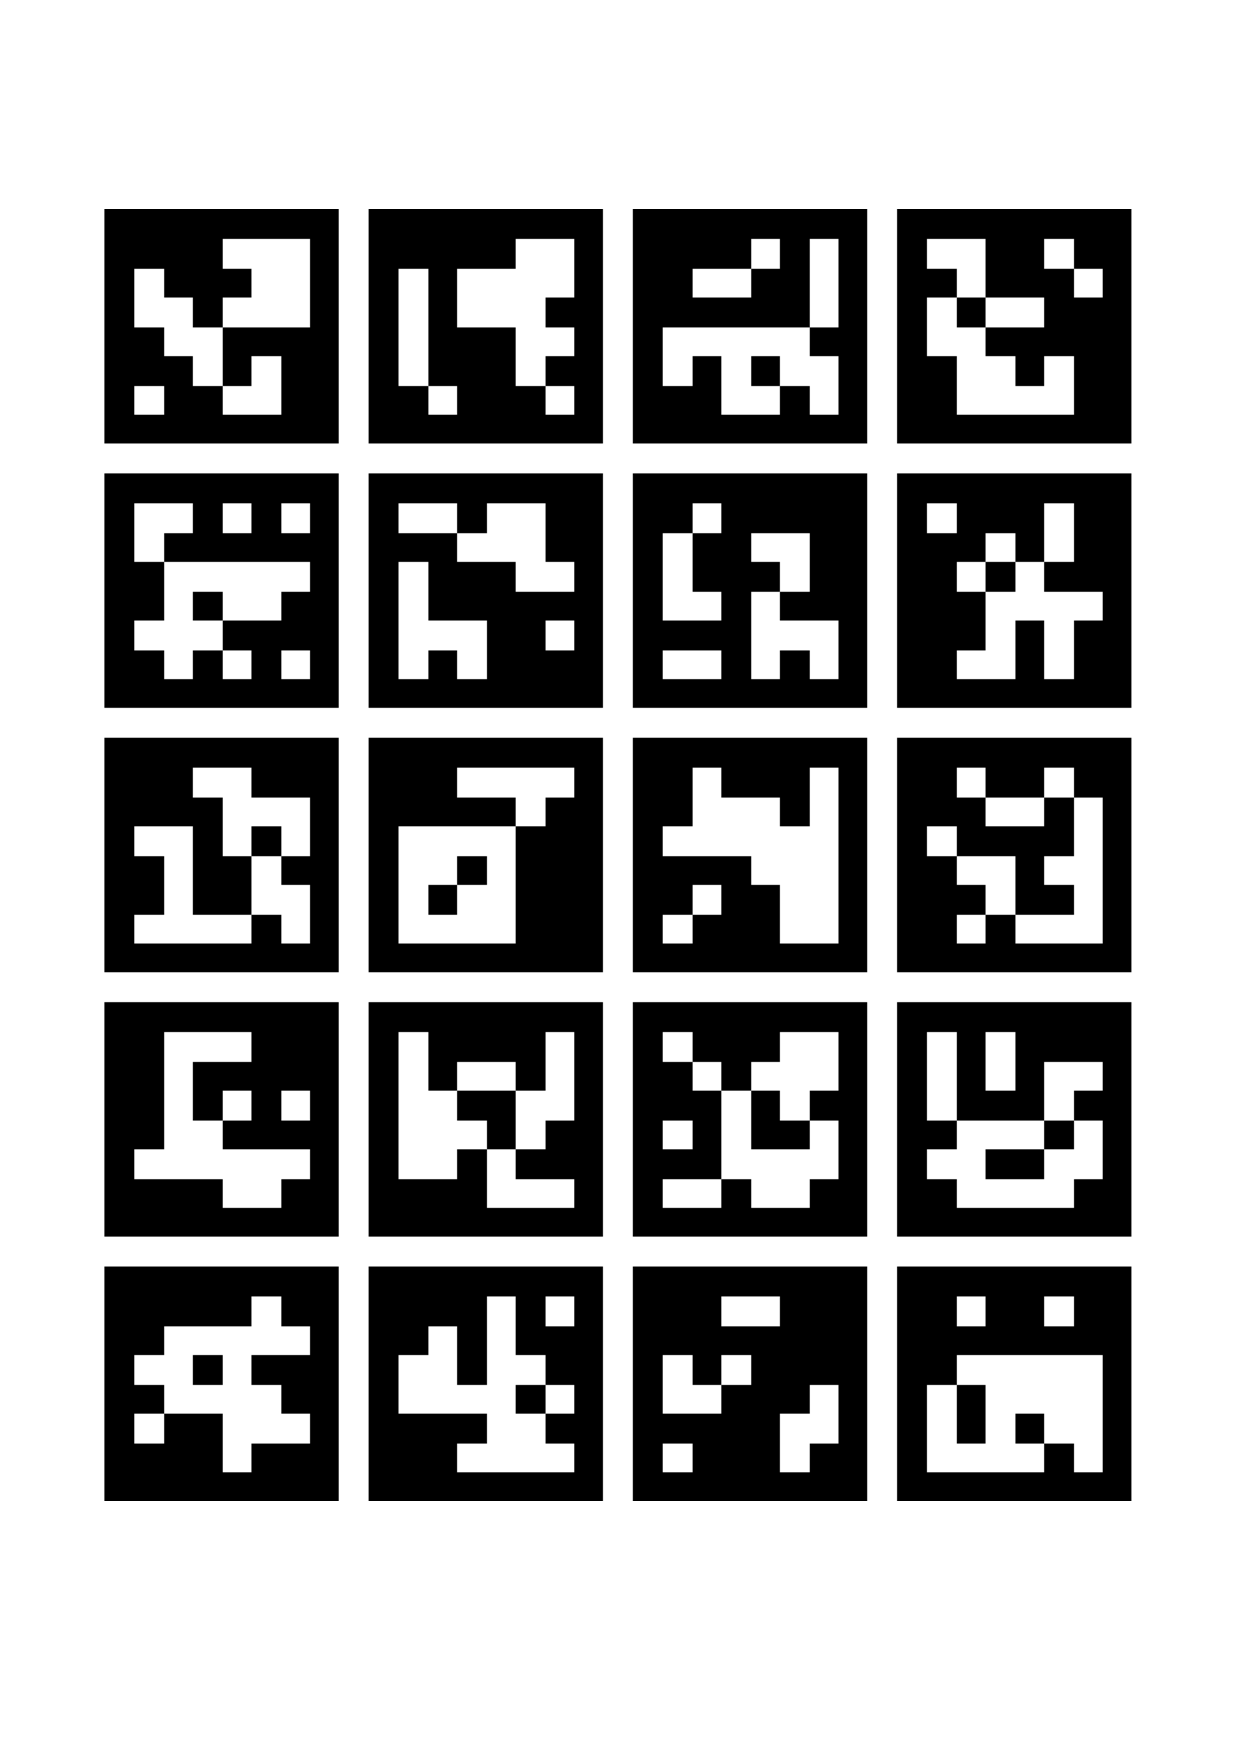
\includegraphics[scale=0.3]{images/aruco_marker_board.pdf}
	\caption{arUco marker board used for demonstrations}
	\label{fig:aruco_marker_board}
\end{figure}

A RGB camera mounted on the robot (mounted on arm in case of KUKA YouBot and mounted on head in case of Toyota HSR) constantly captures images of the arUco marker board which is being moved by teacher for demonstration. Captured images are processed for estimating boards position in camera optical frame. A already available library in opencv is used to estimate the board's 6D pose. Then the estimated pose is transformed to robot's base\_link using transforms published by robot\_state\_publisher. 

\subsection{pydmps}

During this research and development project, the DMP framework described by eq. \ref{DMP_1}, \ref{DMP_2} and \ref{canonical} implemented in open-source project \textit{pydmps}\cite{pydmps}, is used. The original implementation cannot be used for robot control because of following reasons: 
\begin{itemize}
	\item 
\end{itemize} 
